% Created 2020-06-05 Fri 11:56
% Intended LaTeX compiler: pdflatex
\documentclass[11pt]{article}
\usepackage[utf8]{inputenc}
\usepackage[T1]{fontenc}
\usepackage{graphicx}
\usepackage{grffile}
\usepackage{longtable}
\usepackage{wrapfig}
\usepackage{rotating}
\usepackage[normalem]{ulem}
\usepackage{amsmath}
\usepackage{textcomp}
\usepackage{amssymb}
\usepackage{capt-of}
\usepackage{hyperref}
\author{Njagi Mwaniki}
\date{\today}
\title{}
\hypersetup{
 pdfauthor={Njagi Mwaniki},
 pdftitle={},
 pdfkeywords={},
 pdfsubject={},
 pdfcreator={Emacs 26.3 (Org mode 9.2.4)}, 
 pdflang={English}}
\begin{document}

\tableofcontents

\section{RNA Viruses}
\label{sec:org608dc6d}
RNA viral populations don’t exist as a collection of organisms with a single
genome but rather as a quasispecies
(also called a mutant spectrum or a mutant cloud) where most of the biologically
relevant variation observed in vivo is as a result of genetic variation,
competitive selection and random events acting on multiple replicative units.
These quasispecies dynamics have been used to explain the failure of
monotherapy and synthetic antiviral vaccines but have opened new possibilities
for antiviral interventions \cite{domingoViralQuasispeciesEvolution2012}.
These viruses have mutation rates up to a million times higher than their hosts;
rates that are so high it is unlikely for a virus to have an identical RNA
molecule as its immediate progeny \cite{domingoViralQuasispeciesEvolution2012}. 
Negative selection controls this mutation rate and proof that it is not 
optimized by natural selection is that in some cases it leads to local
extinction \cite{duffyWhyAreRNA2018}.

\subsection{Respiratory Syncytial Virus (RSV)}
\label{sec:orgdd5a84d}
RSV is the major cause of acute lower respiratory tract infections associated 
with pneumonia, bronchitis (Borchers et al., 2013; Zlateva et al., 2004) and
otitis (Klein et al., 1982) more frequently than any other agent and
particularly in the first year of life (Stott \& Taylor, 1985).
As if that wasn’t enough, RSV significantly increases the prevalence of asthma
in children who are hospitalized with it and there is a marked correlation
between the incidence of RSV in the community and the occurrence of sudden
infant deaths as well as a third of cot deaths among children over 3 months of
age (Chanock et al., 1957). 

A simple upper respiratory illness in immunocompromised adults or the elderly
is no longer viewed as trivial (Chanock et al., 1957; Whimbey \& Ghosh, 2000).
People with cardiopulmonary diseases and immunocompromised persons with bone
marrow transplant patients prior to marrow engraftment are at highest risk for
pneumonia and death (Morris et al., 1956). For cancer patients, the risks and
benefits of administering intensive chemotherapy in the setting of a seemingly
benign upper respiratory illness are now weighed heavily (Klein et al., 1982).

In animals, the RSV virus is also recognized as an important cause of Bovine
Respiratory Disease (BRD) in Europe and the United States
(Whimbey \& Ghosh, 2000) being the most costly disease of beef cattle in
North America (Griffin, 1997).

\subsubsection{History}
\label{sec:org970828c}
The virus was first isolated in 1956 from Chimpanzees and named Chimpanzee
Coryza Agent (Morris et al., 1956) after which it was isolated in children from
whom it had not been possible to isolate and renamed RSV in 1957 then
classified in order Mononegavirales, family Paramyxoviridae, subfamily
Pneumovirinae, genus Pneumovirus
(Beem et al., 1960; Chanock et al., 1957; Zlateva et al., 2005).

\subsubsection{Epidemiology}
\label{sec:org8f28fd7}
In older children and healthy adults, RSV presents in highly seasonal annual
epidemics (Aamir et al., 2013; Al-Toum et al., 2006) of mild reinfections
predominantly in the upper respiratory tract (Chanock et al., 1957) even in the
presence of pre-existing antibodies (Cane, 2001; Sullender et al., 1991).

The epidemics have been found to have a significant negative correlation with
temperature and a significant positive correlation with relative humidity and
rainfall (Al-Toum et al., 2006) and therefore crop up in the coldest months
which naturally vary with latitude.

In temperate climates, RSV epidemics occur in the winter between December and
February but peaking in January and February  (Al-Toum et al., 2006) and are a
major cause of winter mortality associated with 60-80\% more deaths than
influenza (Nicholson, 1996).

In tropical climates, epidemics occur during the rainy season
(Aamir et al., 2013; Al-Toum et al., 2006) but are also associated with 
religious festivals (Cane, 2001).

Serious disease is limited to the primary infection which occurs between six
weeks and two years of age during the child’s first or second epidemics
(Cane, 2001) and can occur in the presence of maternally derived antibodies.
However, infants with more severe illnesses were found to have lower levels of
antibodies in serum collected near the onset of illness than did infants with
milder illnesses (Cane, 2001; Glezen et al., 1981).

\subsubsection{The Genetic Makeup of RSV}
\label{sec:org26d5b08}
\begin{figure*}
\centering
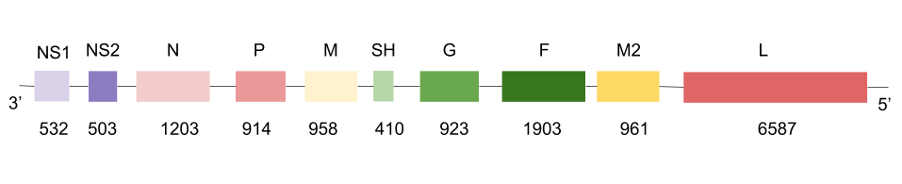
\includegraphics[width=0.7\textwidth]{figures/RSV-genes.png}
\caption{\label{fig:orgc911253}
A schematic of RSV antisense RNA strand showing its 10 genes. The rectangles represent genes with the different shades of the same colour used to show similarity. The grey connectors are the intergenic regions. The numbers below are the estimated gene lengths. Adapted from (Nam \& Ison, 2019)}
\end{figure*}

\begin{figure*}
\centering
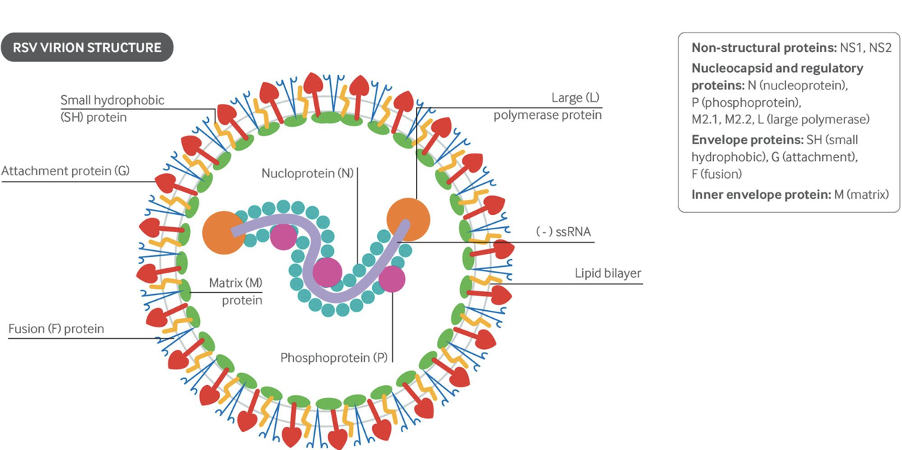
\includegraphics[width=0.7\textwidth]{figures/RSV-cross-section.png}
\caption{\label{fig:org440f0f9}
A schematic of the RSV capsid showing the lipid bilayer and most importantly the surface the F and G glycoproteins. From (Nam \& Ison, 2019).}
\end{figure*}

RSV, whose genome structure is shown above, is an enveloped virus with a
nonsegmented negative-strand RNA genome of approximately 15,200 nucleotides
containing 10 genes which code for 11 proteins whose order is 3k NS1, NS2, N,
P, M1, SH, G, F, M2 (note that M2 codes for M2.1 and M2.2 proteins), and L with
attenuation of transcription step-wise with distance from the 3k end
(Cane, 2001).

As shown in table 1 and figures 1 and 2, RSV has three surface glycoproteins:
the small hydrophobic (SH) protein which may be non-structural, the fusion (F)
protein which plays the main role in virus penetration, syncytium formation,
and possibly can also mediate attachment and the attachment (G) glycoprotein
which plays the main role in virus attachment. It has four nucleocapsid
proteins including the nucleoprotein (N), phosphoprotein (P),
M2-1(also designated 22K and sometimes considered a matrix protein) and
polymerase (L). 
The M2 gene contains a second open reading frame encoding a protein (M2-2) which
regulates transcription (Fearns \& Collins, 1999). There is a single matrix 
protein, M1, which may mediate interactions between the nucleocapsid and
envelope and the two non-structural proteins, NS1 and NS2  have recently been 
shown to antagonise the interferon-induced antiviral response
(Fearns \& Collins, 1999; Schlender et al., 2000).
\subsubsection{Groups of RSV}
\label{sec:org5a6c65e}
RSV was initially divided into two antigenic groups A and B in 1966 by its 
reaction with panels of monoclonal antibodies particularly those directed
against its P, F and G proteins (Coates et al., 1966). It is worth noting that
only antibodies directed against the G and F proteins have been shown to be
neutralising in vitro or protective in vivo (Cane, 2001). 

It was later demonstrated that the two groups are distinct at the genetic level
(Philip R. Johnson \& Collins, 1988). The F and N proteins are highly conserved
between the groups showing 91\% and 96\% amino acid similarity, respectively 
(Philip R. Johnson \& Collins, 1988, 1989). In contrast, the G protein was found
to be highly variable where the amino acid similarity of this protein between
groups A and B was 53\% (P. R. Johnson et al., 1987; Zlateva et al., 2004).

Both groups are known to circulate within an epidemic (T. C. Peret et al., 1998)
without any leading to the extinction of the other, although A tends to be more
dominant in epidemics attributed to the higher variability among the A strains
(T. C. Peret et al., 1998; Zlateva et al., 2005).

The sequence diversity of the G glycoprotein (the type II glycoprotein of
289–299 amino acids depending on the virus strain (Cane, 2001) coded by the 
G gene suggests that the two subgroups have evolved separately for a significant
period of time with proof of RSV A’s most recent common ancestor dating back as
the early 1940s (Zlateva et al., 2004).

Because the F gene mutates at a much lower rate compared to the G gene it
becomes an adequate vaccine target which is why we talk of RSV F vaccines 
(Anderson et al., 2013; Giersing et al., 2016). This lower rate of mutation also
leads to consistent identification by antibodies and therefore the major
neutralizing antibody response to RSV appears to be induced by the F protein 
(Olmsted et al., 1986).

Groups A and B are subdivided further into subgroups, as of 2012 there were 11
subgroups of RSV A: ON1, GA1–GA7, SAA1, NA1, and NA2 and 17 subgroups of RSV
B: GB1–GB4, SAB1-SAB3, and BA1–BA10 
(Aamir et al., 2013; Eshaghi et al., 2012; T. C. Peret et al., 1998; T. C. T. Peret et al., 2000; Shobugawa et al., 2009; Trento et al., 2003, 2006; Venter et al., 2001).

\section{Graphs in Bioinformatics}
\label{sec:orgb48db45}
Contemporary methods of representing a reference genome as a linear sequence of 
characters to represent bases \cite{diltheyImprovedGenomeInference2015} introduce a
mapping bias towards alleles in the reference known as reference bias compared
to the mapping of alternative alleles
\cite{degnerEffectReadmappingBiases2009,brandtMappingBiasOverestimates2015}. 

This naturally leads to a need for a structure that can represent variation that
is inherent in the genome. Other models can approach this structure with
varying degrees of accuracy, but it is naturally represented as a graph in
which the sequences themselves are implicitly encoded as walks in the graph
\cite{patenGenomeGraphsEvolution2017}.
\section{Graph Theory}
\label{sec:orgc36073d}
A graph is an object, or collection, of two sets, a vertex set and edge set.
The vertex set is a finite non-empty set, to mean a graph must have at least one
vertex.
The edge set may be empty \cite{trudeauIntroductionGraphTheory1993}
and is used to present relationships between the vertices.

More formally, a graph G is an unordered pair (V(G), E(G)) consisting of a set
V(G) of vertices and a set E(G), disjoint from V (G), of edges, together with
an incidence function that associates with each edge of G an unordered pair of
(not necessarily distinct) vertices of G \cite{bondyGraphTheory2011}.

Graphs can be represented diagrammatically as shown below.
G \{\{a c\} \{b d\}\}
\begin{figure*}
\centering
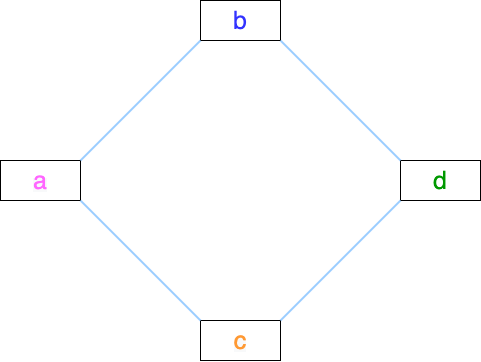
\includegraphics[width=0.7\textwidth]{figures/Graph-classifications-Undirected.png}
\caption{\label{fig:orgd70b6b5}
G is an undirected graph of four nodes a,b,c and d.}
\end{figure*}


H \{\{a c\} \{c d\}\}
\begin{figure*}
\centering
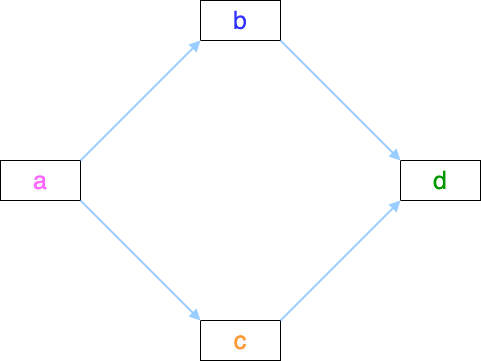
\includegraphics[width=0.7\textwidth]{figures/Graph-classifications-Digraph.png}
\caption{\label{fig:orgf3e7416}
H is an undirected graph of notes a, b and c. Two vertices which are incident with a common edge are adjacent, as are two edges which are incident with a common vertex, and two distinct adjacent vertices are neighbours \cite{bondyGraphTheory2011}.}
\end{figure*}


\subsection{Graph classifications}
\label{sec:org60ba7db}
Graphs can be broken down into many classifications but in this case, we want to
focus on simple versus multigraphs and directed versus undirected.
A simple graph can only have one edge connecting two adjacent vertices while a
multigraph is a graph in which two adjacent vertices are connected by more than
one edge.

Simple Graph
\begin{figure*}
\centering

\includegraphics[width=0.7\textwidth]{figures/Graph-classifications-Simple-Graph.png}
\caption{\label{fig:org3a2cd54}
A simple graph showing only a single edge connecting any two nodes}
\end{figure*}


Multigraph
\begin{figure*}
\centering
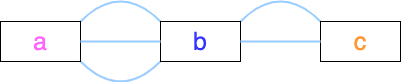
\includegraphics[width=0.7\textwidth]{figures/Graph-classifications-Multigraph.png}
\caption{\label{fig:org2f6fadd}
A multigraph where more than one edge can connect any two nodes.}
\end{figure*}


Figure 3: (a) A simple graph showing only a single edge connecting any two
nodes. (b) A multigraph where more than one edge can connect any two nodes.
A directed graph also called a digraph is a graph in which the edges have
direction.

Figure 4: A directed graph with the edges indicating direction.
An undirected graph is one in which the edges do not have direction indicated on
them.

Figure 5: An undirected graph where the edges have no indication of direction.
A bidirected graph is one in which each edge has an independent orientation
\cite{edmondsMatchingWellSolvedClass2003}.
This is important for the representation of strand, that is reading a DNA
molecule in its forward or reverse complement orientation 
\cite{patenGenomeGraphsEvolution2017}.

The degree of a vertex v in a graph G, is the number of edges of G incident with
v (going in and out of v), each loop counting as two edges. In directed graphs,
we have the concept of indegree and outdegree. The indegree refers to the
numbers of head ends of the edges adjacent to a vertex and the outdegree is the
number of tail ends of the edges adjacent to a vertex \cite{bondyGraphTheory2011}.
A vertex is even if its degree is an even number and odd otherwise
\cite{trudeauIntroductionGraphTheory1993}.

An isomorphism is a relationship between two graphs such that the two graphs
can be represented by identical diagrams \cite{bondyGraphTheory2011} whereas an 
automorphism of a graph is an isomorphism of the graph to itself as shown below.

\begin{figure*}
\centering
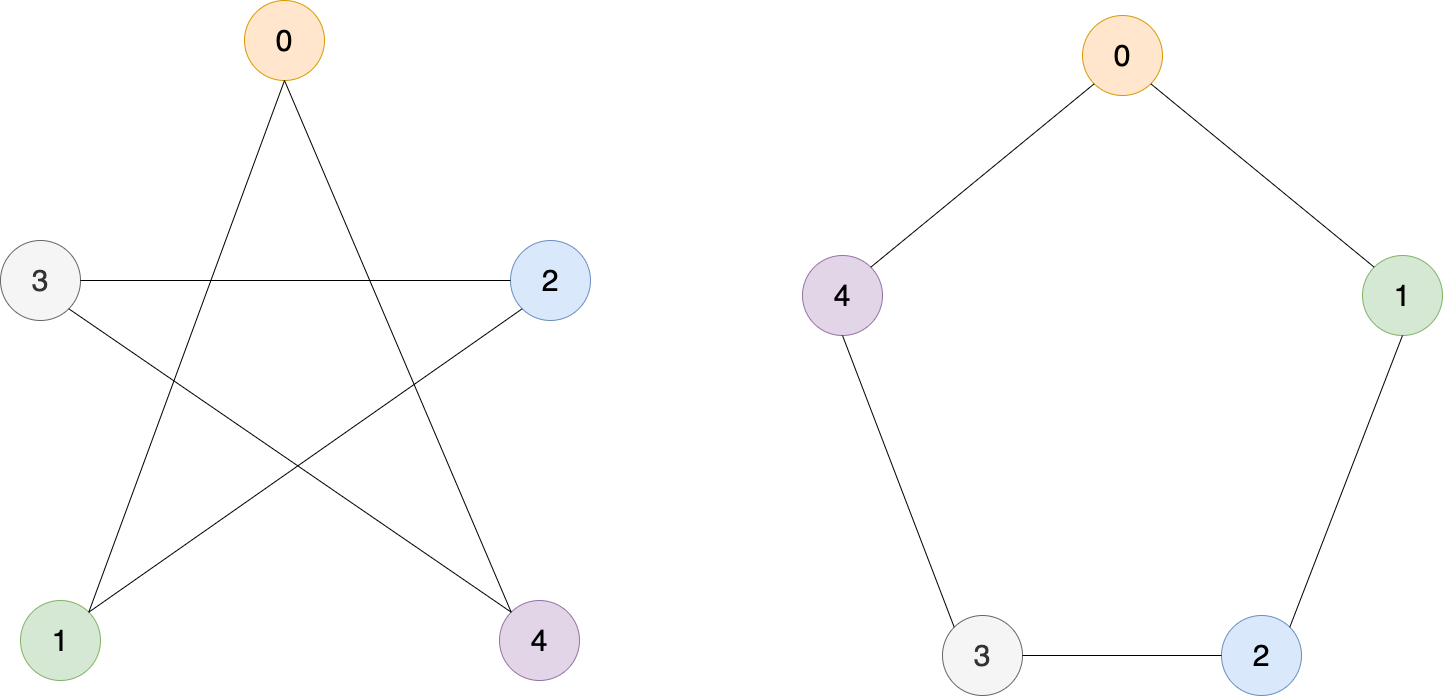
\includegraphics[width=0.7\textwidth]{figures/Isomorphism.png}
\caption{\label{fig:org5ff67e4}
The two nodes are different visualizations of the same graph and therefore an isomorphism.}
\end{figure*}

\subsection{Walks and paths}
\label{sec:org634474c}
A path is a simple graph whose vertices can be arranged in a linear sequence in
such a way that two vertices are adjacent if they are consecutive in the 
sequence, and are nonadjacent otherwise \cite{bondyGraphTheory2011}.

A walk in a graph is a sequence A1 A2 A3 \ldots{} An of not necessarily distinct 
vertices in which A1 is joined by an edge to A2, A2 is joined by an edge to
A3, \ldots{}, and An−1 is joined by an edge to An. The walk A1 A2 A3 \ldots{} An is said
to join A1 and An \cite{trudeauIntroductionGraphTheory1993}.

Therefore, a path is a graph, whereas a walk is a traversal of a graph.

An Euler or Eulerian walk is a walk that uses every edge in the graph exactly
once.

A Hamiltonian walk is like an eulerian walk but for nodes and can be open or
closed, an open hamilton walk is a walk that uses every vertex in the graph
exactly once. A closed hamilton walk is a closed walk that uses the initial
vertex exactly twice and all the other vertices in the graph exactly once
\cite{trudeauIntroductionGraphTheory1993}.

\section{Genome Graphs}
\label{sec:org1442992}
A genome graph is a generic term that refers to the representation of a sequence
or sequences or genetic material using graph-based methods implicitly or
explicitly. Genome graphs are expected to lead to improvements in mapping reads,
variant calling and haplotype determination \cite{patenGenomeGraphsEvolution2017}.

Genome graphs are generally directed graphs and have different classifications,
based on where the sequences are held within the graph, either on the edge or in
the nodes.

These are vertex-labelled directed graphs, graphs whose nodes are labelled such
that a directed walk can be interpreted as a DNA sequence, defined by the
sequence of node labels along the walk and edge-labelled directed graphs in
which case the nodes, rather than the edges, can be viewed as representing the 
intersection points between connected subsequences
\cite{patenGenomeGraphsEvolution2017}.

\subsection{De Bruijn Graph}
\label{sec:org53b642c}
These are graphs used in the assembly of reads named after Dutch mathematician
Nicolaas de Bruijn who became interested in the superstring problem: find a 
shortest circular superstring that contains all possible substrings of length k
(k-mers) over a given alphabet which he solved using an eulerian walk over the
k-mers \cite{compeauHowApplyBruijn2011}.

\subsection{Sequence graph}
\label{sec:org9622695}
A sequence graph is a bidirected graph in which each node is labelled with a
nucleotide string a “sequence graph” \cite{patenGenomeGraphsEvolution2017}.
In this bidirected graph, the features of an edge indicate to which side of a 
node (sequence), 5’ or 3’, each end of the edge connects" \cite{novakGenomeGraphs2017}.

\subsection{Variation Graph}
\label{sec:org68723c2}
A variation graph is a graph where a complete walk along the graph represents a
haplotype \cite{patenGenomeGraphsEvolution2017}.

Many genome graphs don’t represent the concept of the strand, "reading a DNA
molecule in its forward and reverse complement orientations". To express
strandedness, directed graphs can be generalized to bidirected graphs
\cite{edmondsMatchingWellSolvedClass2003,medvedevComputationalMethodsDiscovering2009}
in which each edge endpoint has an independent orientation, indicating whether 
the forward or the reverse complement strand of the attached node is to be
visited when entering the node through that endpoint of the edge.
Inversions, reverse tandem duplications, and arbitrarily complex rearrangements
are expressible in the bidirected representation
\cite{patenGenomeGraphsEvolution2017}.

\subsection{Population Reference Graphs (PRGs)}
\label{sec:orgdc026fd}
Population reference graphs are graphs that represent a population-wide genome
combining multiple reference sequences and catalogues of variation
\cite{diltheyImprovedGenomeInference2015}. 
This concept may also be extended to represent, in our case, a virus mutant
cloud.

\subsection{Problems arising from graph-based reference models}
\label{sec:org5800a4a}
\subsubsection{Calling alleles at sites}
\label{sec:orgd196a0a}
This involves declaring an allele at a given position, this position could span
several nodes or edges in an undefined manner. 

A proposed way to describe their positions is via motif
\cite{patenGenomeGraphsEvolution2017}, patterns of interconnections occurring
in complex networks at numbers that are significantly higher than those in
randomized networks \cite{miloNetworkMotifsSimple2002}, called a superbubble in directed graph
or an ultrabubble in bidirected graphs \cite{patenSuperbubblesUltrabubblesCacti2017}.

Superbubbles and ultrabubbles are directed acyclic subgraphs that connect to the
rest of the graph through one source node and one sink node
\cite{patenSuperbubblesUltrabubblesCacti2017}.
\subsubsection{Non-trivial indexing and reference mapping}
\label{sec:orgbfaea9f}
We now need to use methods that are aware of alternative alleles to map reads to
a graph reference \cite{patenGenomeGraphsEvolution2017}. 
The indexing could be done through gbwt \cite{sirenHaplotypeawareGraphIndexes2018}
could be achieved via partial order alignment gssw \cite{zhaoSSWLibrarySIMD2013}.
\subsubsection{Coordinate system}
\label{sec:org4d4c7e3}
A reference genome coordinate system is a system that uses coordinates to
uniquely determine the positions of bases in the reference genome 
\cite{randCoordinatesIntervalsGraphbased2017}.

An interesting problem introduced by graph-based reference structures is that
it’s no longer trivial to define a locus on the reference
\cite{patenGenomeGraphsEvolution2017}. The Computational Pan-Genomics
Consortium (2016) however agreed on qualities that a coordinate system should 
have \cite{patenGenomeGraphsEvolution2017,randCoordinatesIntervalsGraphbased2017}.
A coordinate system should have: monotonicity genome graph coordinates of
successive bases within a genome should be increasing, legibility coordinates 
should be compact and human interpretable, spatiality bases physically close
together within a genome should have similar coordinates, vertical spatiality
of bases that are allelic variants of one another
\cite{randCoordinatesIntervalsGraphbased2017}. 
horizontal spatiality of bases that can appear together within a single molecule
\cite{randCoordinatesIntervalsGraphbased2017}.
\subsection{Mapping reads to a reference genome graph}
\label{sec:org4e1dd7f}
Given that a genetic sequence is read in small pieces for short reads and much
longer pieces for long reads, we need to find where in the genome a read comes
from. Read mapping is the process of finding the position where the read came
from in a reference sequence or graph \cite{novakGenomeGraphs2017}.
\subsubsection{Reference bias or reference allele bias}
\label{sec:org9820eea}
Reference allele bias is the tendency to under-report data whose underlying DNA
does not match a reference allele \cite{patenGenomeGraphsEvolution2017}.
Masking known SNP positions in the genome sequence can eliminate the reference
bias but do not lead to more reliable results overall
\cite{degnerEffectReadmappingBiases2009}.

\subsection{Variation Graphs in Virus Haplotype Detection and Quantification}
\label{sec:orge3ae7b2}
Compared to eukaryotes, viruses have relatively short genomes and high mutation 
rates \cite{duffyWhyAreRNA2018} and RNA viruses exist as a quasi-species 
\cite{domingoViralQuasispeciesEvolution2012}. This gives rise to the need to
deconvolute the individual haplotypes and quantify them.

There are a number of other tools for the assembly of haplotypes of virus
quasispecies.
These can be broadly categorized into reference-guided and reference-free.
De novo approaches do not require any prior information, such as a reference
genome or knowledge of the quasispecies composition. De novo approaches have
been shown to have advantages over reference-guided reconstruction, since using
a reference genome can induce significant biases
\cite{baaijensStrainawareAssemblyGenomes2020}.

There exist methods for de novo, strain aware metagenomic assembly such as 
VG-flow \cite{baaijensStrainawareAssemblyGenomes2020} however which focus only on 
short-read data.
VG-flow takes as input a next-generation sequencing (NGS) data set and a 
collection of strain-specific contigs assembled from the data and produces 
full-length haplotypes and corresponding abundance estimates 
\cite{baaijensStrainawareAssemblyGenomes2020}.
\end{document}
